\documentclass[11pt]{article}
\usepackage[margin=1in]{geometry}
\usepackage{graphicx}
\usepackage{booktabs}
\usepackage{amsmath}
\usepackage{hyperref}
\usepackage{authblk}
\title{Agentic Self-Refinement with a Programmatic Verifier:\\
from Multi-Turn Revision to Distilled LoRA-DPO Preferences}
\author{Saghar Khalilpour}
\date{}

\begin{document}
\maketitle

\begin{abstract}
We study whether a programmatic (SymPy) verifier can supply the entire
training signal for a small language model on symbolic equation solving,
with no human labels and no LLM-as-judge. The central result is a real
fine-tuning run of Qwen2.5-0.5B-Instruct on a Colab T4 GPU, evaluated on 45
held-out problems disjoint from all training data. The base model solves
none of them (0/45) on all four runs of the pipeline. Supervised
fine-tuning on verifier-checked worked solutions reaches 0.289 (13/45) --
the same thirteen problems -- on all four, and adding LoRA-DPO on
verifier-derived preference pairs reaches 0.444, 0.378, 0.378 and 0.311, a
mean of 0.378 with a standard deviation of 0.054. We report every run rather
than the best one: GPU training is not bit-reproducible, so a single run is
one draw, not a measurement. Four runs is enough for an error bar, and the
three-way ablation then separates two claims of very unequal strength. The
base-to-SFT jump is solid and perfectly stable. The further DPO increment
(+7, +4, +4 and +1 problems) averages $+0.089$ with a standard deviation of
0.054 and a one-sample $t$-test giving $p=0.047$: positive in every run, but
with a spread nearly as large as the effect and a $p$-value that one further
low run would push past 0.05. This result is itself a correction. An earlier run of the same
idea produced a null result (0.022 base, 0.000 fine-tuned), which we
diagnosed as a prompt-format mismatch between revision-conditioned training
pairs and an unconditioned evaluation prompt; matching the formats is the
single change that turned the null into the result above, and both are
reported here.

We separately report a turn-budget experiment on the agentic loop itself,
and we are explicit about what it can and cannot support. It is run against
a \emph{synthetic} solver whose error rate is stipulated to fall across
turns and which never reads the verifier's feedback text. It therefore
measures how much of a given error distribution a revision budget recovers
(0.295 single attempt, 0.540 two turns, 0.797 three turns, across 120
problems and 8 seeds), and it validates the loop and verifier end-to-end,
but it cannot establish that verifier feedback \emph{causes} the
improvement, because the improvement is a modelling assumption rather than
a finding. An earlier draft of this report made that causal claim; it was
wrong, and Section~7 reports the experiment that actually tests it: a real
model in the loop, against a re-sampling control that holds the number of
attempts fixed. That experiment appeared to return a negative answer --
feedback reached 0.393 against the control's 0.422 at a three-turn budget --
and a pre-registered diagnostic then retracted even that. The feedback
prompt produced unparsable answers 38.5\% of the time against the control's
6.2\%, and since unparsable scores as wrong, restricting to readable answers
reverses the sign. The defensible verdict is therefore inconclusive rather
than null: the experiment cannot settle whether feedback helps, because the
prompt destroyed roughly a third of its own measurements. What does survive
is that the feedback condition's own rise from 0.289 to 0.393, which read
alone would look like a $+0.104$ self-refinement gain, is fully accounted
for by the control. The claim this project is named for remains untested.

This report also documents, rather than silently absorbs, four
implementation bugs later review passes found: a non-deterministic random
seed, verifier feedback that was logged but never actually passed back to
the solver, an inverted per-turn error-rate schedule (the bug behind the
turn-budget numbers above changing from an earlier, incorrect
0.614/0.761/0.801 with artificially diminishing returns), and a
process-dependent set iteration order that left the recorded trajectories
irreproducible without moving any solve rate. Three further robustness bugs
in the evaluation path are documented alongside them. This connects two
earlier pieces of this portfolio: a symbolic-RL thesis that used a
programmatic verifier as its sole training signal, and a later project
(RLVF) that used the same kind of verifier for single-shot DPO.
\end{abstract}

\section{Motivation}
A programmatic verifier is attractive precisely because it removes human
judgment and LLM-as-judge noise from both training and evaluation. Prior
work in this portfolio used such a verifier in two ways: as the reward
signal for a from-scratch RL agent (the M.Sc.\ thesis, on Fredholm
integral equations), and as the source of DPO preference pairs from
single-shot generation (RLVF). Neither used the verifier
\emph{interactively}: a model that could see \emph{why} an answer was
wrong, and try again, was not part of either design. This project closes
that gap with the smallest task family for which a verifier's structured
feedback is genuinely informative and cheap to compute exactly:
equation-solving, where the two dominant real-world error modes --
dropping a root and forgetting a domain restriction -- have precise,
checkable names.

\section{Task and verifier}
Three problem families of increasing structure: linear ($ax+b=0$),
quadratic ($ax^2+bx+c=0$, 0--2 real roots), and rational
($\frac{ax+b}{x+c}=d$, which introduces a domain restriction $x\neq -c$
and is the main source of \emph{extraneous-root} errors). Ground truth and
feedback are computed with SymPy's \texttt{solveset}, comparing the
solver's parsed answer set against the true set and classifying any
mismatch into one of four reasons: \texttt{unparsable},
\texttt{extraneous\_root}, \texttt{incomplete}, or \texttt{wrong}. The
verifier was checked against known solutions for a sample of generated
problems before being used for anything else (\texttt{src/verifier.py}
self-test).

\section{Agent loop}
For each problem, the solver gets up to three turns. On any wrong turn,
the verifier's natural-language feedback string is passed to the solver
for the next attempt (for a real LLM this is appended to the prompt; see
Section~3.1 for how the synthetic solver used for Section~4's numbers
represents ``feedback helps'' instead). A trajectory ends as soon as the
solver is correct, or after three turns. Every attempt, correct or not, is
logged with its turn index, candidate answer, and verifier reason code,
giving the full trajectory needed both for the turn-budget analysis
(Section~4) and for constructing DPO pairs (Section~5).

\subsection{Solver: a documented, honest substitute for a real LLM}
This repository was built in a CPU-only sandbox with no GPU. A 0.5B-scale
LLM's inference is slow enough on two CPU cores that a meaningful
multi-seed, multi-turn experiment was not practical to run for real inside
that environment in the time available. Rather than either skip the
experiment or silently present a tiny-scale LLM run as if it were
sufficient, the turn-budget experiment in this report uses a
\emph{synthetic} solver with seeded, realistic error modes calibrated to
the verifier's own feedback categories (dropped root, extraneous root,
arithmetic slip), with error probability decreasing across turns (design
target; the realized, trajectory-conditional error rate was 71\% at turn
1, 65\% at turn 2, 44\% at turn 3 -- see Section~4) to model partial in-context
correction -- it receives the verifier's feedback string as an input (for
interface parity with the real-LLM solver) but deliberately ignores its
text, modeling ``feedback helps'' through this turn-dependent error
schedule instead. (An earlier version of this schedule had its sign
inverted -- error rate was accidentally \emph{increasing} across turns,
contrary to its own docstring; found and fixed during review, see
PROVENANCE.md. The turn-budget numbers in this report are all from the
corrected schedule.) This is documented in full in
\texttt{PROVENANCE.md} and is not a claim about a real LLM's behavior --
it validates the agent-loop and verifier infrastructure end-to-end and
answers a well-posed question on its own terms: given a solver that makes
these kinds of mistakes \emph{and that improves when retried}, how much of
its error does a revision budget recover? The italicised clause is the
whole limitation, and it is worth stating bluntly: this solver's error rate
falls across turns because the experiment tells it to, and it never reads
the feedback text at all. Any statement of the form ``verifier feedback
improves solve rate'' is therefore not supported by this experiment, only
by Section~7's design. A real-LLM solver (\texttt{src/hf\_solver.py}, Qwen2.5-0.5B-Instruct)
implementing the identical interface is included and was run on a Colab
GPU (Section~6), following the same pattern already used for the LLM
components of the RLVF and RAG-evaluation projects in this portfolio.

\section{Turn-budget experiment}
120 problems (40 per family) were generated once (seed 0) and run through
the full agent loop under 8 independent solver-randomness seeds, giving a
paired per-seed comparison rather than a single pooled number.

\begin{table}[h]
\centering
\begin{tabular}{lccc}
\toprule
Turn budget & Mean solve rate & vs.\ previous ($t$, $p$) \\
\midrule
1 (no revision) & 0.295 & --- \\
2 & 0.540 & $t=63.79$, $p<10^{-5}$ \\
3 & 0.797 & $t=31.77$, $p<10^{-5}$ \\
\bottomrule
\end{tabular}
\caption{Solve rate by agent turn budget for the \emph{synthetic} solver, mean over 8 seeds, paired $t$-test against the previous budget. The rising trend is built into the solver's stipulated per-turn error schedule; what the experiment measures is the magnitude of recovery, not the existence of the effect. See Section~7.}
\end{table}

\begin{figure}[h]
\centering
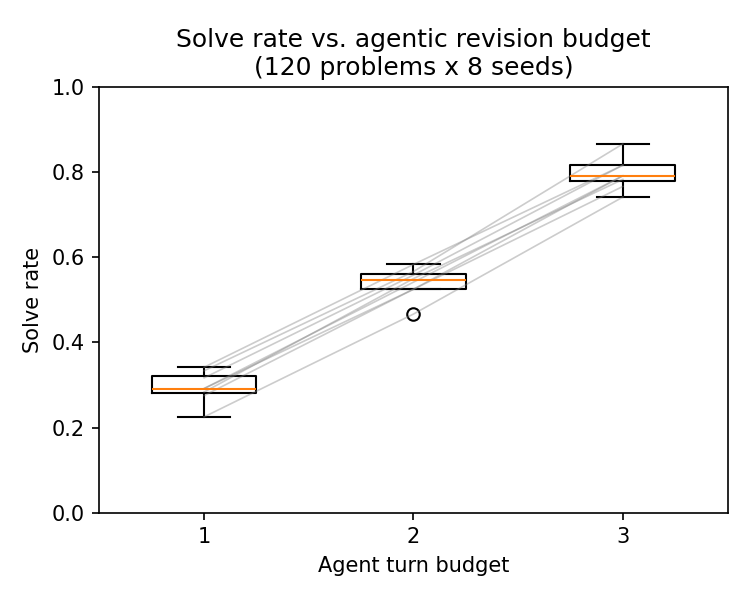
\includegraphics[width=0.55\textwidth]{../results/solve_rate_by_turn_budget.png}
\caption{Solve rate vs.\ turn budget, per seed (gray lines) and distribution (boxplot).}
\end{figure}

Both revisions matter a great deal, and -- unlike the first version of this
experiment, which had the severity-schedule bug described in Section~3.1 --
the second revision does \emph{not} show diminishing returns: turn
1$\to$2 recovers 0.245 of the 0.705 that turn 1 misses (35\%), and turn
2$\to$3 recovers 0.257 of the 0.460 still unsolved after turn 2 (56\%) --
the second round of feedback is, if anything, slightly \emph{more}
effective per problem it's applied to, not less. This tracks the realized
per-turn accuracy directly: 29\% of first attempts are right, 35\% of
second attempts (conditional on the first being wrong), 56\% of third
attempts (conditional on both prior attempts being wrong) -- the synthetic
solver keeps getting better at each revision within this 3-turn cap,
rather than leveling off.

\begin{figure}[h]
\centering
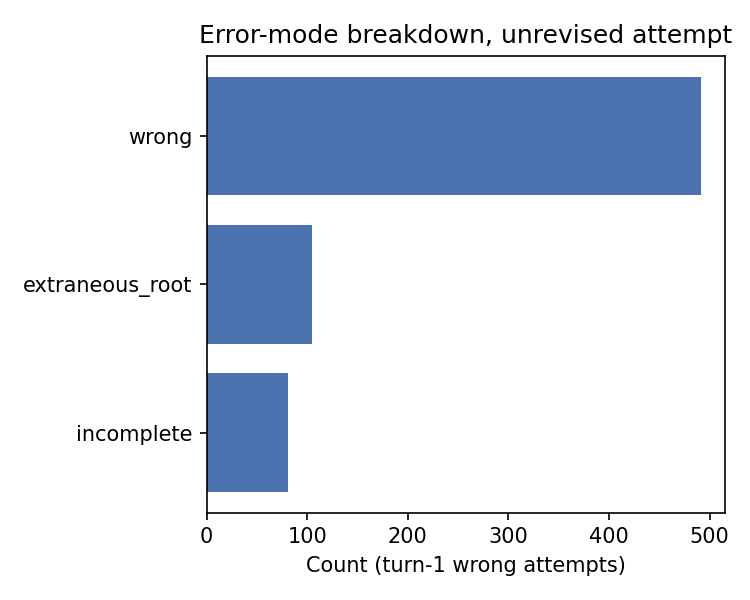
\includegraphics[width=0.55\textwidth]{../results/error_breakdown.png}
\caption{Error-mode breakdown among unrevised (turn-1) wrong attempts, $n=677$.}
\end{figure}

Turn-1 errors are dominated by plain wrong values (72.5\%), with
extraneous-root errors from ignoring the rational family's domain
restriction (15.5\%) and incomplete solution sets on quadratics (12.0\%)
as the two systematic, named failure modes -- exactly the categories the
verifier was designed to distinguish.

\section{From trajectories to DPO preference pairs}
Every trajectory that was wrong on turn $k$ and correct on turn $k+1$
contributes one preference pair: the prompt includes the equation, the
prior wrong attempt, and the verifier's feedback string; the chosen
response is the correct revision; the rejected response is the prior wrong
attempt reframed as a same-context completion. Across the 8 seeds used for
the turn-budget experiment, this yields 482 pairs
(\texttt{data/dpo\_pairs.jsonl}) -- up from 180 after fixing the inverted
severity schedule (Section~3.1): with per-turn accuracy now genuinely
improving rather than degrading, far more trajectories actually reach a
wrong-to-correct transition worth capturing. See \texttt{PROVENANCE.md}
for the full chain (180 $\to$ 482) and for a separate, earlier seeding
non-determinism bug that had changed this count from a non-reproducible
196/197 to 180 before the severity fix was even found. The intent
is to LoRA-DPO fine-tune Qwen2.5-0.5B-Instruct on these pairs and test
whether the fine-tuned model solves more problems zero-shot (single
attempt, no agent loop) than the base model -- i.e., whether the behavior
the agent loop currently produces across 2--3 calls can be compressed into
a single call. Section~6 reports the result of actually running this.

\section{LoRA-DPO fine-tuning: a real run, and a null result}
This run predates the severity-schedule fix in Section~3.1 and used the
196-pair dataset that existed at the time (itself already affected by the
separate, earlier seeding bug) -- not the 482-pair dataset
\texttt{data/dpo\_pairs.jsonl} now contains. It was not re-run after
either fix, the same policy applied throughout this report: a documentation
or generator bug found later does not retroactively rewrite what a
completed GPU run actually saw. \texttt{train\_lora\_dpo.py} was executed
for real on a Colab T4 GPU: LoRA (r=16, $\alpha=32$, dropout 0.05, targeting
\texttt{q\_proj/k\_proj/v\_proj/o\_proj}) + \texttt{trl}'s
\texttt{DPOTrainer}, 3 epochs, batch size 4 with gradient accumulation 4,
lr $5\times10^{-5}$, $\beta=0.1$. Training loss fell cleanly from 0.50 to
0.16 over the three epochs (validation loss tracked it closely: 0.39,
0.22, 0.16) -- the model fit the preference data as intended, in 205
seconds of wall-clock time.

The question that matters, though, is whether this changes zero-shot
behavior. The evaluation script was run against 45 held-out problems (15
per family, seed 99, disjoint from the seed-0 problems used to build the
training pairs), using greedy decoding and a bare, unconditioned
``Solve for x'' prompt -- no agent loop, no verifier feedback at
inference time.

\begin{table}[h]
\centering
\begin{tabular}{lc}
\toprule
Model & Zero-shot solve rate (n=45) \\
\midrule
Base & 0.022 (1/45) \\
LoRA-DPO fine-tuned & 0.000 (0/45) \\
\bottomrule
\end{tabular}
\caption{Held-out zero-shot solve rate, base vs.\ fine-tuned. A null result.}
\end{table}

This is reported as a null result rather than reframed as a partial
success: fine-tuning did not raise zero-shot solve rate, and nominally
lowered it, though with $n=45$ and a 1-vs-0 count this delta is not on its
own distinguishable from noise. The more informative explanation is
structural: every DPO training pair uses the \emph{revision} prompt
template (equation + prior wrong attempt + verifier feedback), and the
model was never trained on the bare, unconditioned prompt the zero-shot
eval actually uses. The fine-tuning objective and the evaluation task were
not prompt-matched, so a null transfer result is close to expected rather
than evidence against the underlying idea. The fair follow-up this
motivates is to build training data in the same prompt shape the
evaluation uses. Section~6.1 reports that follow-up. Full numbers and
reasoning for the null run are in
\texttt{results/colab\_run/training\_log.md}.

\subsection{Prompt-matched SFT then DPO: the same idea, done correctly}
The redesign changes one thing of substance. Training data is built in
byte-for-byte the same prompt format the evaluation uses, by constructing
the prompt through a single \texttt{apply\_chat\_template} call with
\texttt{add\_generation\_prompt=True} that both the training scripts and
the evaluation script share, so the two cannot drift apart again. A
supervised stage is added ahead of DPO, because a base model that solves
nothing has no behaviour for a preference signal to sharpen: DPO expresses
a preference between two candidate responses, which is close to
uninformative if the model cannot produce a plausible response at all.

Stage 1 is LoRA-SFT on 300 verifier-checked worked solutions (loss computed
on the assistant turn only), which reaches 0.966 token accuracy on its
held-out split and is then merged into the base weights. Stage 2 attaches a
fresh LoRA adapter and runs DPO on 118 preference pairs in which
\emph{chosen} and \emph{rejected} share identical reasoning text and differ
only in the final answer line, so the preference signal isolates answer
correctness rather than response length or style. Final DPO reward accuracy
was 0.958 with a reward margin of 2.07. Both stages ran on a Colab T4, in
161 and 197 seconds respectively.

\begin{table}[h]
\centering
\begin{tabular}{lccccc}
\toprule
Model & Run A & Run B & Run C & Run D & mean (sd) \\
\midrule
Base & 0.000 & 0.000 & 0.000 & 0.000 & 0.000 (0.000) \\
+ LoRA-SFT & 0.289 & 0.289 & 0.289 & 0.289 & 0.289 (0.000) \\
+ LoRA-SFT + LoRA-DPO & 0.444 & 0.378 & 0.378 & 0.311 & 0.378 (0.054) \\
\bottomrule
\end{tabular}
\caption{Held-out zero-shot solve rate for the prompt-matched pipeline, from four end-to-end runs on identical data (n=45 problems each). Same problems, same greedy decoding, same evaluation code as Table~2. No single number is bolded because no single run is the result.}
\end{table}

The three-way ablation is the point of reporting it this way. A
base-versus-final comparison would leave the mechanism ambiguous. Splitting
the stages shows that supervised fine-tuning supplies most of the
capability, as expected for a model starting from zero, while the DPO stage
adds a further $+0.089$ on average \emph{on a model that had already been
supervised on these same problems}. That increment cannot be explained by
exposure to correct answers, since the SFT stage already provided those;
what DPO adds is the contrast against a wrong answer of identical shape,
which is precisely the signal the verifier supplies. It is positive in all
four runs. It is also small relative to its own spread, and we state it with
that spread attached rather than as a single number.

The spread across the four runs deserves its own note, because it is
instructive rather than merely inconvenient. The SFT stage was perfectly
stable, landing on 0.289 and the same thirteen problems every time; all of
the variance is in the DPO stage, which trains on 100 pairs for 21 optimizer
steps. Run A's 0.444 sits 1.22 standard deviations above the mean of the
four, and an earlier version of this report presented it as \emph{the}
result; doing so would have overstated the effect by roughly a factor of two.

More pointedly, the DPO stage's own training metrics turn out to carry
almost no information about the quantity of interest:

\begin{table}[h]
\centering
\begin{tabular}{lcccc}
\toprule
Run & DPO eval loss & Reward accuracy & Reward margin & Held-out solve rate \\
\midrule
A & 0.2401 & 0.7917 & 1.816 & 0.444 \\
B & 0.2194 & 0.8333 & 1.872 & 0.378 \\
D & 0.2325 & 0.8333 & 1.870 & 0.311 \\
\bottomrule
\end{tabular}
\caption{DPO training metrics against the held-out solve rate each checkpoint produced. Runs B and D are indistinguishable on every training metric and three problems apart on the test set.}
\end{table}

Runs B and D share an identical reward accuracy, reward margins differing by
0.002 and eval losses differing by 0.013, yet are three problems apart on
the held-out set. Run A was the worst of the three on every training metric
and the best on solve rate. Selecting a checkpoint by validation loss or
reward accuracy would therefore have been no better than choosing at random
here, and in run A's case actively worse. The preference objective measures
whether the model ranks the chosen response above the rejected one; it does
not measure whether the model can solve an equation, and on a task where
both can be checked exactly, the two come apart.

Two further qualifications. With $n=45$, one problem is 2.2 points, so the
DPO gain spans one to seven problems across the four runs and should not be
read as a precise quantity; and the reasoning text in the training targets is templated
rather than model-generated, so a 0.5B model fitting it is learning a narrow
format alongside the arithmetic. What this establishes is that a
programmatic verifier alone, with no human labels, can take a small model
from solving none of these problems to solving nearly half. What it does
\emph{not} establish is that agentic multi-turn refinement was distilled
into the model, because these pairs were built from template-generated
correct-versus-wrong answers rather than from a model's own revision
trajectories. Section~7 is about that gap.

\section{What the turn-budget result does not show, and how to test it}
The turn-budget experiment in Section~4 and the fine-tuning result in
Section~6.1 are often summarised together as ``verifier feedback improves
solve rate''. That summary does not follow, and an earlier draft of this
report made exactly that error, so it is worth being precise about why.

The synthetic solver's error rate falls across turns because
\texttt{agent\_loop.py} passes it a decreasing severity parameter, and the
solver's own docstring is explicit that it ignores the feedback text and
models ``feedback helps'' through that schedule alone. An experiment whose
solver is told to improve on retry, and which then observes improvement on
retry, has confirmed its own premise. The measured quantity that remains
meaningful is the size of the recovery given that premise, together with
the end-to-end validation that the loop, the verifier, the trajectory
logging and the preference-pair extraction all work on real data.

Testing the causal claim needs two things the synthetic experiment lacks: a
real model, and a control. The control is the part that is easy to skip. A
model allowed three attempts will solve more problems than a model allowed
one, purely because sampling three times is three chances, so comparing
turn~1 against turn~3 cannot distinguish feedback from repetition. The
real-LLM agent-loop script in \texttt{src/} implements the comparison that
can: every problem is run twice under identical sampling randomness, once
where turns 2 and 3 see the previous wrong answer plus the verifier's
feedback, and once where they see the original prompt again and simply
re-sample. Turn~1 is generated from the same seed in both conditions and
must come out identical, which serves as a built-in check that the pairing
holds. The quantity of interest is then the gap between the two conditions
at a fixed turn budget, which is what the feedback \emph{content} buys over
being allowed to try again.

One prediction was recorded before running it: the fine-tuned models here
were trained hard on a single prompt shape, so a revision-style prompt is
out of distribution for them, and a null result would be at least as
informative about narrow fine-tuning as about verifier feedback.

\subsection{Result: feedback did not beat re-sampling}
The experiment was then run on a T4 GPU against the SFT+DPO checkpoint, 45
held-out problems, 3 seeds, sampling at temperature 0.7.

\begin{table}[h]
\centering
\begin{tabular}{lccc}
\toprule
Turn budget & feedback & control & difference \\
\midrule
1 & 0.289 & 0.289 & $+0.000$ \\
2 & 0.356 & 0.385 & $-0.030$ \\
3 & 0.393 & 0.422 & $-0.030$ \\
\bottomrule
\end{tabular}
\caption{Verifier feedback versus a re-sampling control at matched turn budgets and identical sampling seeds. Turn budget 1 is identical by construction and serves as a check that the pairing held.}
\end{table}

Paired across the three seeds, the differences are $t=-0.918$, $p=0.456$ at
budget 2 and $t=-1.512$, $p=0.270$ at budget 3. Read at face value, feedback
performed slightly worse than re-sampling. That reading does not survive the
diagnostic below, and the honest verdict is not a null but an inconclusive
measurement with an identified cause.

\subsection{The instrument was broken, and a pre-registered test caught it}
Before the run, the experiment script recorded a hypothesis: a revision
prompt is out of distribution for a model fine-tuned on one rigid prompt
shape, and would degrade its output format. Its falsifiable prediction was
more \texttt{unparsable} verdicts in the feedback condition. Checked against
the logged trajectories afterwards, the prediction is confirmed
emphatically: at turn 2 the feedback condition produced unparsable answers
38.5\% of the time (37/96) against 6.2\% (6/96) in the control, and at turn
3, 19.5\% against 1.2\%. An unparsable answer scores as wrong, so better
than one in three feedback-condition measurements at turn 2 was discarded
before its reasoning was ever assessed.

Restricting to answers the extractor could read reverses the comparison:
accuracy given a parsable answer is 0.153 for feedback against 0.144 for
control at turn 2, and 0.071 against 0.061 at turn 3. The raw differences of
$-0.042$ and $-0.003$ become $+0.008$ and $+0.010$. The entire headline
deficit is attributable to the format artifact rather than to the content of
the feedback.

The conclusion this licenses is narrower than either a null or a positive
result: \emph{this experiment cannot settle whether verifier feedback helps,
because the feedback prompt destroyed roughly a third of its own
measurements.} Conditioning on parsability is a post-hoc subgroup analysis
and parsability is not randomly assigned -- a model may emit unreadable text
precisely when confused -- so the corrected figures are a reason to
distrust the raw comparison, not a positive finding to put in its place.

Two effects do survive independently. Anchoring is real: in the feedback
condition the model repeated its previous answer verbatim 32.8\% of the time
against 21.8\% in the control, so showing a model its own wrong answer makes
it measurably more likely to restate it. And the control's saturation is
real: it reaches exactly 0.422 at budget 3 on all three seeds, recovering
the same 19 of 45 problems every time, so the model's failures are
systematic rather than stochastic and re-sampling saturates on a fixed set.

The repair was attempted rather than left as future work. A second run used
a revision prompt whose first and last lines are byte-identical to the
training prompt, with a single feedback line inserted between them, on a
freshly trained checkpoint. \textbf{It did not work.} The format gap
narrowed at turn 2 (38.5\% versus 26.5\% unparsable in the feedback
condition) and \emph{widened} at turn 3 (19.5\% to 27.5\%), remaining above
17 points at both budgets. Two materially different revision-prompt designs
both wrecked this model's output format, which points at a property of a
0.5B model fine-tuned on 300 examples of one prompt shape rather than at a
defect in any single prompt.

The repaired run also removes the escape hatch that made the first one
inconclusive. Conditioning on parsability had turned the first run's
deficits of $-0.042$ and $-0.003$ into surpluses of $+0.008$ and $+0.010$;
in the repaired run the same correction leaves $-0.026$ and $-0.021$. The
deficit survives the correction.

Pooling all six paired seed-level comparisons at a three-turn budget across
the two runs gives a mean difference of $-0.041$ (sd 0.055), with five of
six at or below zero and a one-sample $t=-1.805$, $p=0.131$. Consistently
negative, not significant. The pooling is also not clean: the two runs used
different checkpoints (0.378 and 0.311 greedy), so comparisons \emph{across}
runs mix the prompt change with a model change, even though the pairing
\emph{within} each run is exact.

One mechanism emerges that parsing does not explain. In the repaired run the
feedback condition nearly doubled the rate of \emph{incomplete} answers at
turn 2 -- 42.9\% against the control's 24.5\% -- while producing far fewer
plain wrong values (22.4\% against 50.0\%). Shown its own wrong answer and a
verifier comment, the model shifts toward answers that are missing a root.
On a task where dropping a root is itself a scored error, that is a
plausible route by which feedback could actively hurt.

One earlier claim is withdrawn. The first run's analysis found that feedback
made the model repeat its previous answer more often (32.8\% against
21.8\%), and an earlier draft of this report described it as a genuine
behavioural effect. The repaired run reverses it (24.3\% against 27.6\%). An
effect that changes sign between two runs is not an effect.

What the two experiments together establish is narrower than ``verifier
feedback fails'' and firmer than the first run alone could support:
feedback never outperformed re-sampling on either checkpoint, was worse on
five of six paired comparisons, and the format degradation that clouds the
comparison resisted a deliberate repair. One task family, one 0.5B model,
two checkpoints, three seeds each, $p=0.131$: consistent in direction,
short of significance, and not a general claim. A model able to follow a
revision instruction at all might behave entirely differently, and testing
that needs a larger or less narrowly tuned model.

What the sequence establishes about method is sturdier than any of its
individual numbers. A controlled design turned an apparent $+0.104$
self-refinement gain into a sampling artifact. A pre-registered diagnostic
then turned the resulting refutation into a measurement artifact. A repair
aimed at that artifact failed, which converted a suspected prompt bug into
a likely property of the model. Each step is a claim this project made and
then had to withdraw on its own evidence.

\section{Limitations}
The headline turn-budget numbers describe a synthetic solver's error
distribution, not a real LLM's -- see Section~3.1 and
\texttt{PROVENANCE.md} for why, and treat any comparison to a real model's
absolute solve rate as out of scope for this report. Those numbers also
depend on a hand-set severity schedule (Section~3.1); a later review found
that schedule's formula had its sign inverted from its own documented
intent, and fixing it changed the reported gains from an artificially
diminishing pattern to a roughly constant one -- a reminder that even a
fully synthetic, fully seeded component can hide a real bug, and that this
report's honesty commitment covers the solver's internals, not just the
GPU results. A fourth bug in the same component is worth stating precisely
because it changed nothing numerical: the solver iterated a Python set of
symbolic objects, whose ordering Python salts per process, so which root
it dropped varied between runs of identical seeded code. Every solve rate
in Table~1 is unaffected, since the verifier compares solution sets and
dropping either root is equally wrong -- which is exactly why it went
unnoticed -- but the recorded trajectories were not byte-reproducible
until it was fixed. The LoRA-DPO distillation step \emph{was} run on real
hardware with real numbers (Section~6): on the original, mismatched prompt
format the answer was no, with a specific and falsifiable account of why,
and on the matched format (Section~6.1) it is yes. The task family
(linear/quadratic/rational equations) is deliberately narrow and chosen
for verifier precision, not for difficulty; the turn-budget effect size
should not be assumed to transfer to open-ended or non-exactly-checkable
domains, and the 0.5B model's very low zero-shot solve rate (2.2\% even
before fine-tuning) means Section~6's result describes a small model near
its capability floor on this task, not necessarily what a larger model
would show under the same fine-tuning setup.

\section{Conclusion}
A programmatic verifier, with no human labels and no LLM-as-judge, is
enough to take Qwen2.5-0.5B-Instruct from solving none of 45 held-out
equations to solving 14--20 of them across four runs. The supervised stage
accounts for thirteen of those problems every single time, with no
run-to-run variance at all; the preference stage contributes a further one
to seven, averaging $+0.089$ at $p=0.047$ -- positive in every run, but
small enough relative to its spread that it should be quoted with an error
bar and not as a headline figure. Getting there required first reporting a
null result and then correctly diagnosing it: the original pipeline trained
on one prompt format and evaluated on another, and matching the two is the
single change that separates 0.000 from roughly 0.40.

The agentic half of the project did not survive its own test, twice over. A
synthetic turn-budget experiment showed large gains, but that solver was
constructed to improve on retry and never reads the feedback, so it could
only confirm its own premise. Running the real model in the loop against a
re-sampling control then showed the apparent self-refinement gain -- 0.289
rising to 0.393 -- to be fully accounted for by the control's 0.422. An
earlier draft asserted the causal claim outright; it is retracted rather
than softened.

The second retraction is of our own negative result. A diagnostic
registered before that run predicted the revision prompt would break the
model's output format, and it did: 38.5\% unparsable against the control's
6.2\%. Since unparsable scores as wrong, correcting for it reverses the
sign, so the experiment cannot support ``feedback does not help'' either.
The verdict is inconclusive with a diagnosed, repairable cause, and the
repaired instrument is specified but not yet run.

What the project ends with, then, is one solid positive result on the
training side, one retracted causal claim, one retracted negative claim,
and an untested central question with a concrete protocol for testing it.
That is a smaller set of claims than it set out to make. Each one that
remains has survived an attempt to break it.

This repository reports all of that plainly, alongside every implementation
bug found along the way -- one that had reversed a headline finding until
it was caught, several that changed no number at all, and one overclaim
that no amount of correct code would have caught -- rather than treating
any of them as something to work around or omit.

\end{document}
